107. $(|x-2|-1)(y+x^2-2x-3)=0\Leftrightarrow\left[\begin{array}{l}|x-2|=1,\\y=-x^2+2x+3.\end{array}\right.\Leftrightarrow
\left[\begin{array}{l}x=3,\\x=1\\y=-x^2+2x+3.\end{array}\right.$
$$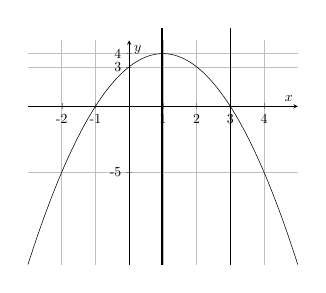
\begin{tikzpicture}[scale=0.5]
\tikzset {line01/.style={line width =0.5pt}}
\begin{axis}[
    axis lines = middle,
    grid=major,
    legend pos={south west},
    xlabel = {$x$},
    ylabel = {$y$},
    ymin=-12,
    ymax=5,
    xtick={-2,-1,1, 2, 3,4},
    xticklabels={-2,-1,1,2, 3,4},
    ytick={-5,3, 4},
    yticklabels={-5,3, 4}            ]
\addplot[domain=-3:5, samples=100, color=black] {-x*x+2*x+3};
%\addplot[domain=-3.1:2.5, samples=100, color=red] {70*abs(1-2*abs(abs(x)-2))-10*x^2+10*x-70};
	%\addlegendentry{$\text{Рис. 1}$};
\end{axis}
\draw[line01] (3.4,0) -- (3.4,6);
\draw[line01] (5.15,0) -- (5.15,6);
%\draw (3.44,3.185) circle (2pt);
%\draw (3.44,2.5) circle (2pt);
\end{tikzpicture}$$
